
\documentclass[11pt,letterpaper]{article}
\usepackage[spanish]{babel}
%\usepackage[ansinew]{inputenc}
\usepackage[utf8]{inputenc}
% \usepackage[latin1]{inputenc}
\usepackage[letterpaper,includeheadfoot, top=0.5cm, bottom=3.0cm, right=2.0cm, left=2.0cm]{geometry}
\renewcommand{\familydefault}{\sfdefault}

\usepackage{graphicx}
\usepackage{color}
\usepackage{hyperref}
\usepackage{amssymb}
\usepackage{url}
\usepackage{fancyhdr}
\usepackage{hyperref}
\usepackage{subfig}

\usepackage{listings} %Codigo
\lstset{language=SQL, tabsize=4,framexleftmargin=5mm,breaklines=true}

\title{\vspace{-3em}Resumen Exámen DB}
\date{\vspace{-4em}}

\begin{document}
\lstset{language=SQL}
\maketitle
%================================================================
\section{Álgebra relacional}
Existen los siguientes operadores:
\begin{itemize}
	\item $\sigma$ Selecciona filas de una relación. (Es como el WHERE de SQL)
	\item $\pi$ Hace una proyección de las columnas de la relación. (Es como el SELECT de SQL)
	\item $\cup$ Une relaciones, para esto el dominio de las relaciones tiene que ser el mismo. El esquema generado es idéntico al del primer conjunto.
	\item $\cap$ Intersecta relaciones, tienen que ser union-compatible. El esquema generado es idéntico al del primer conjunto.
	\item $-$ Diferencia de relaciones, tienen que ser union-compatible. El esquema generado es idéntico al del primer conjunto.
	\item $\times$ Producto cruz, el esquema generado tiene todos los campos del primer conjunto seguido de todos los del segundo. Contiene todas las combinaciones posibles de los primeros con cada uno de los segundos.
	\item $\rho$ Renombramiento de relaciones, tiene la siguiente forma $\rho (C(1 \rightarrow a, 2 \rightarrow b), R1 \times R2$ lo que hace es que a $R1 \times R2$ lo llama $C$ y las columnas en la posición $1$ y $2$ se llamarán $a$ y $b$ respectivamente en el esquema de $C$ 
	\item  $\Join$ Join de relaciones, es un producto cruz seguido de selecciones y proyecciones. \newline Se cumple $R \Join_c S = \sigma_c( R \times S)$ donde $R,S$ son relaciones y $c$ es una condición. Cuando la condición es una igualdad se llama Equi-Join y cuando la condicion es una igualdad donde ambas columnas tienen el mismo nombre en las relaciones, esta se omite y se llama Natural-Join
	\item $/$ Division, se mostrará como ejemplo.
\end{itemize}
Tomemos las siguientes instancias con el fin de realizar ejemplos:
\begin{table}[h!]
\parbox{.3\linewidth}{
\center
\begin{tabular}{|c|c|c|c|}
	\hline
	sid & sname & rating & age \\ \hline\hline
	28 & yuppy & 9  & 35.0 \\ \hline
	31 & lubber & 8 & 55.5 \\ \hline
	44 & guppy & 5  & 35.0 \\ \hline
	58 & rusty & 10 & 35.0 \\ \hline
\end{tabular}\par
\bigskip
T1
}
\hfill
\parbox{.3\linewidth}{
\center
\begin{tabular}{|c|}
\hline
	age \\ \hline \hline
	35.0 \\ \hline
	
\end{tabular}\par
\bigskip
T2
}
\parbox{.3\linewidth}{
\center
\begin{tabular}{|c|c|}
	\hline
	sname & sex \\ \hline\hline
	yuppy & male \\ \hline
	lubber & female \\ \hline
	guppy & female \\ \hline
	rusty & male \\ \hline
\end{tabular}\par
\bigskip
T3
}
\end{table}

\begin{enumerate}
	\item Seleccionar las filas con rating mayor a 8 en T1: $\sigma_{rating>8}(T1)$
	\item Seleccionar sname y rating en T1: $\pi_{sname,rating}(T1)$
	\item Seleccionar sname y rating de las filas con rating mayor a 8 en T1: $\pi_{sname,rating}(\sigma_{rating>8}(T1))$
	\item Seleccionar sname de las filas con edad 35.0, lo haremos con renombramiento. $\rho(Edad35,\sigma_{age=35.0}(T1)$ y luego $\pi_{sname}(Edad35)$
	\item Seleccionar sname, age y sex de las tablas T1 y T3 uniendo por sname. $\pi_{sname,age,sex}(T1 \Join T3)$
	\item Seleccionar las filas con age 35.0: $T1/T2$
\end{enumerate}
%================================================================
\section{Cálculo relacional}
Ejemplo: Encontrar todas las filas con rating mayor a 8
$\{ R| R \in T1 \wedge R.rating > 8\} $

Definición de fórmula atómica: Sean $Rel$ una relación, $R,S$ tuplas y $c$ una constante, entonces una formula atómica es:
\begin{itemize}
	\item $R \in Rel$
	\item $R.a\textnormal{  op }S.b$
	\item $R.a\textnormal{ op }c$ ó $c\textnormal{ op }R.a$
\end{itemize}

Definición de una formula: Sean $p,q$ fórmulas:
\begin{itemize}
	\item Una fórmula atómica cualquiera
	\item $\neg p$, $p \wedge q$, $p \vee q$ y $p \Rightarrow q$
	\item $\exists R(p(R))$ donde R es una tupla de variables.
	\item $\forall R(p(R))$ donde R es una tupla de variables.
\end{itemize}


%================================================================
\section{Dependencias y Normalización}
\subsection{Dependencia Funcional}
\textbf{Definición :}
Sea $R$ un equema de relación y $X,Y$ conjuntos no vacíos de atributos en $R$. Decimos que una instancia $r$ de $R$ satisface la dependencia funcional $X\rightarrow Y$ si lo siguiente se cumple para cualquier par de tuplas $t1,t2$ en $r$: Si $t1.X = t2.X$, entonces $t1.Y = t2.Y$

Ejemplo de dependencia funcional: $AB \rightarrow C$
\begin{table}[h!]
	\center
	\begin{tabular}{|c|c|c|c|}
	\hline
	 A &  B &  C &  D \\ \hline\hline
	a1 & b1 & c1 & d1 \\ \hline
	a1 & b1 & c1 & d1 \\ \hline
	a1 & b2 & c2 & d2 \\ \hline
	a2 & b1 & c3 & d1 \\ \hline
		
	\end{tabular}
\end{table}

Una llave primaria es un caso especial de dependencia funcional, donde todos las columnas de la relación dependen de la llave.
\\\\
Si se cumple que $X\rightarrow Y$, donde $Y$ es el conjunto de todos los atributos, y existe $V\subset X$ tq $V\rightarrow Y$ se cumple, entonces $X$ es una superllave.
\newpage
\subsubsection{Axiomas de Armstrong, determinan el conjunto de todas las FDs (Su clausura)}
\begin{itemize}
	\item \textbf{Reflexividad} Si $X\supseteq Y$, entonces $X\rightarrow Y$ 
	\item \textbf{Aumentativa} Si $X\rightarrow Y$, entonces $XZ\rightarrow YZ$ para cualquier $Z$
	\item \textbf{Transitiva} Si $X\rightarrow Y$ y $Y\rightarrow Z$, entonces $X\rightarrow Z$ 
\end{itemize}

Es conveniente usar las siguiente reglas adicionales cuando se piensa en la clausura de las dependencias funcionales.
\begin{itemize}
	\item \textbf{Union} Si $X\rightarrow Y$ y $X \rightarrow Z$, entonces $X \rightarrow YZ$
	\item \textbf{Descomposición} Si $X\rightarrow YZ$, entonces $X\rightarrow Y$ y $X \rightarrow Z$,
\end{itemize}

\subsection{Dependencia Multivaluada MVD}
Un atributo implica que otro atributo este dentro de un grupo de opciones \\
\textbf{Ejemplo:}

\begin{table}[h!]
	\center
	\begin{tabular}{|c|c|c|}
	\hline
	 ramo &  profesor &  libro \\ \hline\hline
	 Bases de Datos & Perez 		& Libro1 \\ \hline
	 Bases de Datos & Perez 		& Libro2 \\ \hline
	 Bases de Datos & Gonzales 	& Libro1 \\ \hline
	 Bases de Datos & Gonzales 	& Libro2 \\ \hline
	 Teoria 		& Hevia 		& Libro1 \\ \hline
	 Teoria 		& Hevia 		& Libro3 \\ \hline
	 Teoria 		& Hevia 		& Libro4 \\ \hline
	\end{tabular}
\end{table}

Hay 3 puntos que notar aca:
\begin{itemize}
	\item El esquema esta en BCNF. Por lo tanto no pensaríamos descomponerlo si solo nos preocupamos de las FDs.
	\item Hay redundancia. El dato que Perez enseña Bases de datos esta repetido por cada libro que el ocupa. Ademas el dato de que se puede enseñar Bases de Datos con el Libro1 esta repetido por cada profesor que lo ocupa.
	\item La redundancia podría eliminarse descomponiendo el esquema RPL (Ramo,Profesor,Libro) en RP (Ramo,Profesor) y RL (Ramo,Libro)
\end{itemize}
La redundancia en este ejemplo es debido a la restricción de que los libros por cursos son independientes de los profesores, lo que no puede ser expresado en términos de FDs. \\
Esta restricción es un ejemplo de dependencias multivaluadas.\\ \\
\textbf{Definición:} \\
Sea $R$ una relación y $X,Y$ subconjuntos de atributos de $R$. La dependencia multivaluada $X \rightarrow \rightarrow Y$ pertenece a $R$ si $\forall$ instancia de $R$ cada valor de $X$ es asociado a un conjunto de valores de $Y$ y ese conjunto es independiente de los valores de los otros atributos. \\ \\
\textbf{Formalmente:} \\
Si la MVD $X \rightarrow \rightarrow Y$ pertence a $R$ y $Z = (R-XY)$, entonces $\forall r$ instancia de $R$ si $t_1 \in r$, $t_2 \in r$ y $t_1.X = t_2.X$ entonces debe existir algún $t_3 \in r$ tal que $t_1.X = t_3.X$ y $t_2.Z = t_3.Z$ \\ \\

\textbf{Ejemplo: MVD $X \rightarrow \rightarrow Y$}
\begin{table}[h!]
	\center
	\begin{tabular}{|c|c|c|c|}
	\hline
	 $X$ &  $Y$ &  $Z$ &  \\ \hline\hline
	 $a$ & $b_1$ & $c_1$ & -tupla $t_1$ \\ \hline
	 $a$ & $b_2$ & $c_2$ & -tupla $t_2$ \\ \hline\hline
	 $a$ & $b_1$ & $c_2$ & -tupla $t_3$ \\ \hline
	 $a$ & $b_2$ & $c_1$ & -tupla $t_4$ \\ \hline
	\end{tabular}
\end{table}


\subsubsection{Axiomas de Armstrong para MVD}
Hay tres reglas adicionales que sólo involucran a las MVDs:
\begin{itemize}
	\item \textbf{Complemento} Si $X \rightarrow\rightarrow Y$, entonces $X\rightarrow\rightarrow R-XY$
	\item \textbf{Aumento} Si $X \rightarrow\rightarrow Y$ y $W\supseteq Z$, entonces $WX\rightarrow\rightarrow YZ$
	\item \textbf{Transitividad} Si $X \rightarrow\rightarrow Y$ e $Y \rightarrow\rightarrow Z$, entonces $X \rightarrow\rightarrow (Z-Y)$
	\item \textbf{Replicación} Si $X \rightarrow Y$, entonces $X \rightarrow\rightarrow Y$
	\item \textbf{Unión} Si $X \rightarrow\rightarrow Y$ y existe $W$ tq $W\cap Y$ es vacío, $W\rightarrow Z$, y $Y\supseteq Z$, entonces $X\rightarrow Z$
\end{itemize}

%---------------------------------------
\subsection{Formas Normales}
Toda relación en BCNF esta en 3NF. Toda relación en 3NF esta en 2NF y toda relación en 2NF esta en 1NF.

\subsubsection{1NF}
Cada campo contiene solo valores atómicos, es decir cada campo contiene solo 1 valor.

\subsubsection{2NF}
Las dependencias parciales no están permitidas.

\subsubsection{3NF} 
Sean $R$ una relación, $X$ un conjunto de atributos de $R$ y $A$ un atributo de $R$.
$R$ esta en 3NF si $\forall$ FD (Dependencia Funcional) $X \rightarrow A$ en $R$, se cumple uno de los siguientes:
\begin{itemize}
	\item $A \in X$ (Es decir es una FD trivial)
	\item $X$ es superllave
	\item $A$ es parte de una llave de $R$
\end{itemize}

Sólo hay 3 opciones de FD (Triviales, que una key implique algo, o que algo implique una parte de una key) 
\\\\
Si una FD $X \rightarrow A$ viola 3NF, hay solo 2 posibles casos:
\begin{itemize}
	\item $X$ es un subconjunto de una llave $K$. (En este caso la FD se llama dependencia parcial, y se esta guardando repetidamente el par $(X,A)$)
	\item $X$ no es subconjunto de ninguna llave. (En este caso la FD se llama dependencia transitiva, debido a que tenemos una cadena de dependencias $K \rightarrow X \rightarrow A$)
\end{itemize}

\subsubsection{BCNF (Boyce-Codd Normal Form)}
Libre de redundancia
Sean $R$ una relación, $X$ un conjunto de atributos de $R$ y $A$ un atributo de $R$. 
$R$ esta en BCNF si $\forall$ FD (Dependencia Funcional) $X \rightarrow A$ en $R$, se cumple uno de los siguientes:
\begin{itemize}
	\item $A \in X$ (Es decir es una FD trivial)
	\item $X$ es superllave
\end{itemize}
Ejemplo ilustrativo:
\begin{figure*}[h]
\centering
\fbox{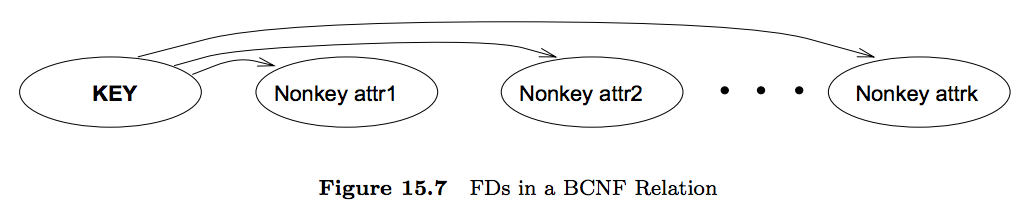
\includegraphics[scale=0.8]{img/ejemplo_bcnf.png}}
\end{figure*}

\subsubsection{Dependencias parciales (S: subconjunto de una llave, X: conjunto de atributos)}
\noindent
Es de la siguiente forma: $S \rightarrow X$.\\
Cumple 3NF pero no BCNF

\subsubsection{Dependencias transitivas (K: llave, X: no es parte de una llave, A: atributo)}\noindent
Es de la siguiente forma: $K \rightarrow X \rightarrow A$.\\
No cumple 3NF ni BCNF

\subsection{Descomposición}
Es una técnica para eliminar redundancia

\subsubsection{Test de descomposición sin perdida}
Sea $R$ una relación y $F$ un conjunto de FD en $R$. La descomposición de $R$ en los conjuntos de atributos $R_1$ y $R_2$ es sin perdida $\Leftrightarrow$ $F$ contiene la FD $(R_1 \cap R_2) \rightarrow R_1$ o contiene la FD $(R_1 \cap R_2) \rightarrow R_2$ \\ \\
Si una FD $X \rightarrow Y$ en una relación $R$ tal que $(X \cap Y)$ es vacío, entonces la descomposición de $R$ en $(R-Y)$ y $XY$ es sin perdida. \\ \\
En BCNF se elimina la redundancia pero se pueden perder FDs \\
En 3NF se elimina parte de la redundancia pero se puede asegurar no perder FDs

\subsection{Normalización}
\subsubsection{Descomposición a BCNF (podrían perderse FDs)}
\begin{enumerate}
	\item Suponemos que $R$ no está en BCNF. Sea $X \subset R$, $A \in R$, y $X\rightarrow A$ una FD que viola BCNF. Descomponemos $R$ en $R-A$ y $XA$.
	\item Si $R - A$ o $XA$ no está en BCNF, descomponemos nuevamente haciendo recursión con el paso $1$
\end{enumerate}
Ejemplo ilustrativo descomposición a BCNF:
\begin{figure*}[h]
\centering
\fbox{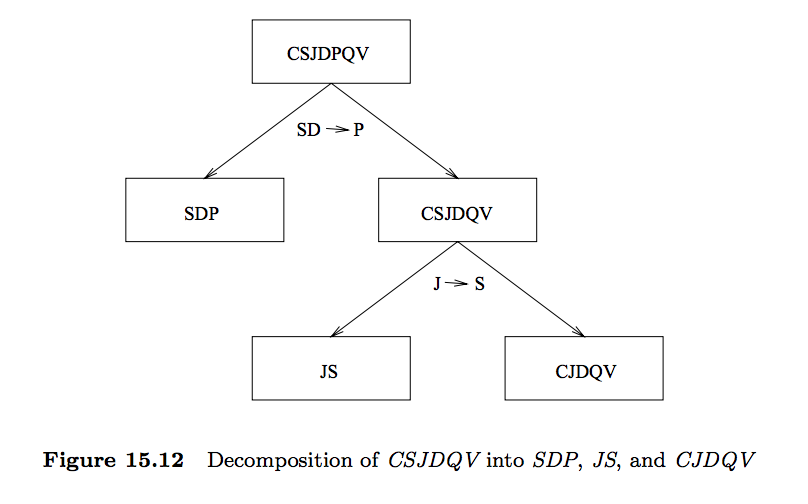
\includegraphics[scale=0.8]{img/ejemplo_descomposicion_bcnf.png}}
\end{figure*}

\subsubsection{Descomposición a 3NF}
\textbf{Minimal Cover (Mínima cantidad de FDs tq la clausura sea la misma que la del conjunto de FDs original}
Un minimal cover para un conjunto $F$ de FDs es un conjunto $G$ de FDs tal que:
\begin{enumerate}
	\item Toda dependencia en $G$ es de la forma $X\rightarrow A$, donde $A$ es un solo atributo.
	\item La Clausura $F+$ es igual a la clausura $G+$
	\item Si obtenemos un conjunto $H$ de FDs borrando una o más dependencias del conjunto $G$, o borrando atributos de una dependencia de $G$, entonces $F+\not = H+$
\end{enumerate}

Intuitivamente, un minimal cover de un conjunto $F$ de FDs es un conjunto de dependencias que es mínimo en dos aspectos:
\begin{enumerate}
	\item Cada dependencia es tan pequeña como es posible; esto es que cada atributo en el lado izquierdo es necesario y que el lado derecho tiene sólo un atributo.
	\item Cada dependencia es necesaria para que la clausura sea igual a $F+$
\end{enumerate}

\textbf{Algoritmo para encontrar minimal cover de $F$}
\begin{enumerate}
	\item Obtener un conjunto $G$ equivalente a $F$ donde todas las FDs tienen sólo un atributo al lado derecho (Usando el axioma de descomposición)
	\item Minimizar el lado izquierdo de cada FD: Para cada FD $g \in G$, revizamos cada atributo del lado izquierdo y vemos si puede ser borrado manteniendo la equivalencia con $F+$.
	\item Borrar FDs redundantes: Revisar cada FD restante en $G$, se borra si se mantiene la equivalencia con $F+$ 
\end{enumerate}

\textbf{Algoritmo para transformar a 3NF}
\begin{itemize}
	\item Identificar el conjunto $N$ de dependencias en $F$ que no cumplen con 3NF 
	\item Para cada FD $X\rightarrow A$ en $N$, crear una relación $XA$ y sumarla a la descomposición de $R$
\end{itemize}

\textbf{Método:} Sea $F$ el conjunto de FDs de una relación $R$
\begin{enumerate}
	\item Obtener el minimal basis (El conjunto $N$ del paso anterior) de $F$, llamémoslo $G$.
	\item Para cada dependencia funcional $X\rightarrow A$ en $G$, usar la relacion $XA$ como parte de la descomposición de $R$.
	\item Si ni uno de los esquemas del paso 2 es una superllave de $R$, añadir una relación cuyo esquema sea una llave de $R$.
\end{enumerate}
\newpage
%================================================================
\section{SQL}
Forma típica de una query en SQL:
\begin{lstlisting}[frame=single]
SELECT [DISTINCT] [column_1] ... [column_n]	
FROM [table_1] ... [table_n]
[WHERE condition_1 ... [AND|OR condition_n]]
[GROUP BY column_1
[HAVING condition_1 ... [AND|OR condition_n]]]
[ORDER BY column_i ASC|DESC]
\end{lstlisting}


%---------------------------------------
\subsection{Create Tables}
Crear una tabla de departamentos
\begin{lstlisting}[frame=single]
CREATE TABLE departamento (
	dep_nom VARCHAR(50),
	fecha_creacion DATE,
	telefono INT,
	direccion VARCHAR(100),
	comuna VARCHAR(20),
	
	PRIMARY KEY (dep_nom)
);
\end{lstlisting}
Crear una tabla empleado que referencia a la de departamentos
\begin{lstlisting}[frame=single]
CREATE TABLE empleado (
	nombre VARCHAR(50),
	depto VARCHAR(50),
	sueldo MONEY DEFAULT 500000,
	fecha_ing DATE NOT NULL,
	
	PRIMARY KEY (nombre),
	
	FOREIGN KEY (depto) REFERENCES departamento(dep_nom) ON DELETE CASCADE,
	
	CHECK (sueldo > 0)
);	
\end{lstlisting}
Las opciones para ON DELETE son:
\begin{itemize}
	\item \textbf{CASCADE} Elimina si se elimina el padre
	\item \textbf{RESTRICT} Detiene la operación de delete en el padre
	\item \textbf{NO ACTION} Lo mismo que RESTRICT
	\item \textbf{SET NULL} Elimina el padre y pone en NULL en la foreign key
\end{itemize}

%---------------------------------------
\subsection{ALTER TABLE}
Se ocupa para modificar una tabla:
\begin{lstlisting}[frame=single]
	ALTER TABLE departamento
		ADD COLUMN jefe VARCHAR(50);
	ALTER TABLE departamento
		ADD FOREIGN KEY (jefe) REFERENCES empleado(nombre);
	ALTER TABLE departamento
		DROP COLUMN jefe;
\end{lstlisting}

%---------------------------------------
\subsection{CREATE INDEX}
Se usa para agregar un INDEX a una tabla
\begin{lstlisting}[frame=single]
CREATE INDEX direccionIndex ON departamento
WITH STRUCTURE = [BTREE|HASH],
KEY = (direccion) 
\end{lstlisting}
%---------------------------------------
\subsection{Queries}
\subsubsection{JOIN}
\begin{itemize}
	\item \textbf{JOIN} Es el producto cruz de las dos tablas, se puede especificar un join condition con la cláusula ON.
	\begin{lstlisting}[frame=single]
		SELECT e.nombre, d.dep_nom, d.telefono
		FROM empleado e JOIN departamento d ON d.dep_nom = e.depto 
	\end{lstlisting}
	\item \textbf{LEFT OUTER JOIN} Es el join entre las tablas, las filas de la primera tabla que no coinciden con alguna de la seguna aparecen igual mostrando NULL en los valores correspondiente a la segunda tabla.
	\item \textbf{RIGHT OUTER JOIN} Análogo al anterior
	\item \textbf{FULL OUTER JOIN} Muestra NULL en todos los que no coinciden en ambos lados.
\end{itemize}
\subsubsection{GROUP BY/HAVING}
	Muestra los departamentos que gastan mas de 5.000.000 en sueldos de sus empleados y el total que gastan.
	\begin{lstlisting}[frame=single]
		SELECT d.dep_nom, SUM(e.sueldo)
		FROM empleado e JOIN departamento d ON d.dep_nom = e.depto
		GROUP BY d.dep_nom
		HAVING SUM(e.sueldo) > 5000000	
	\end{lstlisting}
\subsubsection{UNION/EXCEPT/INTERSECT}
\begin{itemize}
	\item \textbf{UNION} Q1 UNION Q2 entrega los resultados que aparecen en Q1 o en Q2, si hay resultados repetidos sólo se muestran una vez.
	\item \textbf{UNION ALL} Q1 UNION ALL Q2 entrega los resultados que aparece en Q1 o en Q2, si hay resultados repetidos estos se muestran varias veces
	\item \textbf{EXCEPT} Q1 EXCEPT Q2 entrega los resultados que están en Q1 y no en Q2.
	\item \textbf{INTERSECT} Q1 INTERSECT Q2 entrega los resultados que están en Q1 y en Q2
\end{itemize}
\subsubsection{NESTED QUERIES}
\begin{itemize}
	\item \textbf{IN} La condición es que la columna tenga uno de los valores que devuelve Q2
	\begin{lstlisting}
		SELECT ...
		FROM ...
		WHERE column IN (Q2)
	\end{lstlisting}
	\item \textbf{NOT IN} La condición es que la columna \textbf{no} tenga uno de los valores que devuelve Q2
	\begin{lstlisting}
		SELECT ...
		FROM ...
		WHERE column NOT IN (Q2)
	\end{lstlisting}
	\item \textbf{EXISTS} La condición es que Q2 devuelva al menos un resultado
		\begin{lstlisting}
		SELECT ...
		FROM ...
		WHERE EXISTS (Q2)
	\end{lstlisting}
	\item \textbf{ANY/SOME} Que haya algún valor de los resultados de Q2 que cumpla la condición
	\begin{lstlisting}
		SELECT ...
		FROM ...
		WHERE column [=|>|<>|<] ANY (Q2)
	\end{lstlisting}
	\item \textbf{ALL} Que todos los valores de los resultados de Q2 cumplan la condición
	\begin{lstlisting}
		SELECT ...
		FROM ...
		WHERE column [=|>|<>|<] ALL (Q2)
	\end{lstlisting}
	
	También se pueden usar queries anidadas dentro del FROM. Para el HAVING se pueden usar los operadores ANY y EVERY.
\end{itemize}
\subsubsection{LIKE}
Se usa para comparar con strings, tiene los siguientes caracteres especiales:
\begin{itemize}
	\item \textbf{\%} 0 o más caracteres arbitrarios.
	\item \textbf{\_} Exactamente 1 caracter arbitrario.
\end{itemize}
\subsubsection{AGREGATE OPERATORS}
\begin{itemize}
	\item \textbf{COUNT [DISTINCT]} cantidad de valores [únicos]
	\item \textbf{SUM [DISTINCT]} suma de todos los valores [únicos]
	\item \textbf{AVG [DISTINCT]} promedio de los valores [únicos]
	\item \textbf{MAX} máximo entre los valores
	\item \textbf{MIN} mínimo entre los valores
\end{itemize}

%---------------------------------------
\subsection{VIEWS}
Son pseudo-tablas, muestran información de una o más tablas según la query asignada al momento de crearla
\begin{lstlisting}[frame=single]
	CREATE VIEW empleadosRicos (nombre, sueldo)
	AS SELECT e.nombre, e.sueldo
	   FROM empleado e
	   WHERE e.sueldo >= 1000000;
\end{lstlisting}

%---------------------------------------
\subsection{TRIGGERS}
Son acciones que se ejecutan frente a un evento cuando se cumple una condición. 
El siguiente trigger crea una variable y la inicializa en 0 antes de un insert
\begin{lstlisting}[frame=single]
	 CREATE TRIGGER declararVariable
     BEFORE INSERT ON departamentos
  	 DECLARE
     	count INTEGER;
     BEGIN
     	count := 0;
     END
\end{lstlisting}

El siguiente trigger hace que todos los empleados que se ingresen con sueldo menor a 100.000, le asigna 100.000
\begin{lstlisting}[frame=single]
	 CREATE TRIGGER sueldoMinimo
     BEFORE INSERT ON empleado
     FOR EACH ROW
     BEGIN
     	IF NEW.sueldo < 100000 THEN
     		NEW.sueldo = 100000;
     	END IF;
     END
\end{lstlisting}
El siguiente trigger inserta en employee\_tools las tuplas (employee.id, tool.name) donde tool.division = new.division, es decir todas las herramientas correspondientes a la división del empleado.
\begin{lstlisting}[frame=single]
	CREATE TRIGGER employee_INSERT
	AFTER INSERT ON employee
	FOR EACH ROW
	BEGIN
    	INSERT INTO employee_tools (Id, Tool)
    		SELECT NEW.Id, tools.Tool_Name 
            FROM tools
            WHERE tools.Division = NEW.Division;
	END
\end{lstlisting}

%---------------------------------------
\subsection{TRANSACTIONS}
Una transacción es la ejecución de un programa, ya sea de lectura o escritura.
Se usa el acronimo ACID (Atomicity Consistency Isolation Durabilty) para nombrar las cuatro propiedades de una trasacción.
\begin{itemize}
	\item \textbf{Atomicity} Los usuarios no deben preocuparse de los efectos de transacciones incompletas, cada transacción debería ejecutarse sin interferir en las otras, esta labor es del DBMS.
	\item \textbf{Consistency} Cada transacción debería ocurrir de manera no concurrente, el DBMS asume que las transacciones mantienen la consistencia. Por la tanto mantenerla es responsabilidad del usuario.
	\item \textbf{Isolation} El usuario no debe preocuparse de problemas que puedan ocurrir de manera simultanea, el DBMS se encarga de esto.
	\item \textbf{Durability} Cuando el DBMS avisa al usuario que la transacción se realizó adecuadamente, la información debería persistir aunque el sistema se caiga. Claramente el DBMS es responsable de esto.
\end{itemize}

SQL permite al usuario determinar 3 características para una transacción:
\begin{itemize}
	\item \textbf{Access Mode} puede ser READ ONLY que significa que la transacción no puede modificar la DB, o READ WRITE que permite leer y escribir en la DB
	\item \textbf{Diagnostics Size} Determina la cantidad de errores que pueden ser guardados para mostrarlos.
	\item \textbf{Isolation level} Hay cuatro niveles distintos de aislamiento para controlar las transacciones concurrentes. Estos existen para permitir mayor concurrencia aumentando el riesgo de errores. Se especifican abajo.
\end{itemize}

Los niveles de aislamiento, ordenados de mayor aislamiento a menor, son:
\begin{itemize}
	\item \textbf{Serializable} Asegura que la transacción sólo va a leer cambios realizados por otras transacciones commiteadas. Ningún valor que la transacción lea o escriba va a ser cambiado por otra transacción hasta que esta transacción termine. Si la transacción lee un conjunto de valores dependientes de una condición de búsqueda, este conjunto no puede ser modificado por ninguna otra transacción hasta que esta termine.
	\item \textbf{Repeatable Read} Asegura que la transacción sólo va a leer cambios realizados por otras transacciones commiteadas. Ningún valor que la transacción lea o escriba va a ser cambiado por otra transacción hasta que esta transacción termine.
	\item \textbf{Read Commited} Asegura que la transacción sólo va a leer cambios realizados por otras transacciones commiteadas. Ningún valor que la transaccion escriba va a ser cambiado por otra transacción hasta que esta transacción termine. Los valores que se leen podrían ser modificados por otra transacción antes de que esta termine. Está expuesta a phantom read (lecturas fantasmas).
	\item \textbf{Read Uncommited} Los valores leídos pueden ser cambiados por otras transacciones antes de que esta termine. Está expuesta a phantom read. Para usar esta transacción se tiene que estar en ACCESS MODE READ ONLY.
\end{itemize}
%================================================================
\section{XML}

%================================================================
\section{SPARQL}


% ============= FIN DE DOCUMENTO ==============
\end{document}

% % ················ IMAGEN ·················
% \begin{figure}[ht!]
% \centering
% \fbox{\includegraphics[scale=0.6]{img/flujo.png}}
% \caption{Flujo de caja anual}\label{flujo}
% \end{figure}
% %··········································

% % ················ IMAGEN DOBLE ·················
% \begin{figure}[ht!] \centering
% \subfloat[Esquemático]{\includegraphics[scale=0.44]{img/seguidor.png}}
% \subfloat[Simulación]{\includegraphics[scale=0.45]{img/seguidor1.png}}
% \caption{Simulación como seguidor de voltaje}\label{seguidor}
% \end{figure}
% %··········································